\begin{comment}
* Labeling details
- UI, filtering strategy
- Statistics
- Payment
- Timing
- Effectiveness

* General model training
- roberta finetuning
- 4 random seeds
- 3 random samples

* Task 1 - sentiment analysis, generalization accuracy
- 
- 
- 

* Task 2 - NLI, challenge set

* Task 3 - QQP checklist

\end{comment}

\newcommand{\maug}{\texttt{aug}\xspace}
\newcommand{\mcomp}{\texttt{comp}\xspace}

\definecolor{ccon}{HTML}{fee9d4}
\definecolor{cood}{HTML}{d8f0d3}
\definecolor{cid}{HTML}{dae8f5}

\newcommand{\TableAugSST}{
\begin{table*}
\small
\centering
\setlength{\tabcolsep}{4pt}
\begin{tabular}{rrlllllllll}
\toprule
    $n$ &     $m$ &    model & \cellcolor{cid}SST-2 & \cellcolor{cood}Senti140 & \cellcolor{cood}SemEval & \cellcolor{cood}Amzbook & \cellcolor{cood}Yelp & \cellcolor{cood}IMDB & \cellcolor{ccon}IMDB-Cont. & \cellcolor{ccon}IMDB-CDA \\
\midrule
 4,000 &  2,000 &     \mcomp &  $92.9\pm 0.2$ &  $88.9\pm 0.3$ &  $84.8\pm 0.5$ &  $85.1\pm 0.4$ &  $90.0\pm 0.3$ &  $90.8\pm 0.5$ &  $92.2\pm 0.6$ &  $86.5\pm 0.2$ \\
 4,000 &  2,000 &  \maug	 &  $92.7\pm 0.2$ &  $\mathbf{90.7\pm 0.4}$ &  $\mathbf{86.4\pm 0.1}$ &  $85.6\pm 0.8$ &  $90.1\pm 0.0$ &  $90.6\pm 0.3$ &  $\mathbf{94.0\pm 0.3}$ &  $\mathbf{89.7\pm 0.5}$ \\
 % imdb_contrast_test: 91.1 (9.4) / 92.8 (0.4)
 % imdb_contrast_test: 87.4 (0.0) / 89.6 (0.5)
 % imdb_iclr_test 93.0 (0.3) / 93.9 (0.4)
 % imdb_iclr_dev 92.0 (0.2) / 92.7 (0.2)
\bottomrule
\end{tabular}
\caption{\sst model Accuracies on \colbox{cid}{in domain}, \colbox{cood}{out of domain}, and \colbox{ccon}{contrast sets}. \maug performs better than \mcomp on twitter datasets and contrast sets, while maintaining the others.}
\label{table:aug_sst}
\end{table*}}

%%%%%%%%%%%%%%%%%%%%%%%%%%%%%%%%%%%%%%%%%%%%%%%
\newcommand{\TableAugNLI}{
\begin{table*}
\small
\centering
\setlength{\tabcolsep}{4pt}
\begin{tabular}{rrlllllllll}
\toprule
     $n$ &     $m$ &    model & \cellcolor{cid}SNLI & \cellcolor{cood}MNLI-m & \cellcolor{cood}MNLI-mm & \cellcolor{ccon}SNLI-CDA & \cellcolor{ccon}break & \cellcolor{ccon}DNC & \cellcolor{ccon}stress & \cellcolor{ccon}diagnostic \\
\midrule
 20,000 &  1,574 &     \mcomp 	&  $85.7\pm 0.4$&  $86.1\pm 0.2$&  $86.6\pm 0.2$&  $72.8\pm 0.3$&  $86.4\pm 1.5$&  $54.5\pm 0.6$&  $65.1\pm 0.6$&  $56.0\pm 0.8$\\
 20,000 &  1,574 &  \texttt{aug-r} &  $85.7\pm 0.4$ &  $86.1\pm 0.1$ &  $86.2\pm 0.1$ &  $73.4\pm 0.5$ &  $87.2\pm 0.6$ &  $54.7\pm 0.3$ &  $64.6\pm 0.6$ &  $56.9\pm 0.8$ \\
 20,000 &  1,574 &  \maug		&  $85.3\pm 0.3$&  $86.0\pm 0.1$&  $86.4\pm 0.0$&  $\mathbf{73.6\pm 0.2}$&  $\mathbf{89.1\pm 1.2}$&  $\mathbf{57.7\pm 0.3}$&  $65.1\pm 0.2$&  $\mathbf{57.5\pm 0.5}$\\
 %10000 &  1574 &     comp &  $85.3\pm 0.5$&  $85.2\pm 0.2$&  $85.4\pm 0.3$&  $72.4\pm 0.1$&  $86.1\pm 1.8$&  $54.2\pm 1.8$&  $64.0\pm 0.4$&  $56.0\pm 0.3$\\
 %10000 &  1574 &  aug\_gpt &  $85.3\pm 0.3$&  $85.0\pm 0.2$&  $85.1\pm 0.1$&  $73.4\pm 0.5$&  $90.5\pm 1.1$&  $56.5\pm 1.2$&  $64.6\pm 0.5$&  $57.0\pm 0.4$\\
\bottomrule
\end{tabular}
\caption{\nli model Accuracies on \colbox{cid}{in domain}, \colbox{cood}{out of domain}, and \colbox{ccon}{contrast or challenge sets}. \maug performs better than \mcomp on DNC, our targeted contrast set for data-slice-based augmentation. It also improves on other challenge sets.}
\label{table:aug_nli}
\end{table*}
}

%%%%%%%%%%%%%%%%%%%%%%%%%%%%%%%%%%%%%%%%%%%%%%%
\newcommand{\TableAugQQP}{
\begin{table}
\small
\centering
\setlength{\tabcolsep}{4pt}
\begin{tabular}{p{0.4\textwidth} r}
\toprule
TESTNAME &   $\Delta$ fail\%  \\
\midrule
 Order does not matter for symmetric relations &  -18.4\% \\
 Order does not matter for comparison &  -26.5\% \\
 Order does matter for asymmetric relations &  -14.5\% \\
\midrule
 Is it \{ok, bad,..\} to \{smoke, do,..\} \{\emph{before $\not\eq$ after}\} &  -52.5\% \\
 %What was person's life \{\emph{before $\not\eq$ after}\} becoming X &  -46.6\% \\
 Do you have to X your dog \{\emph{before $\not\eq$ after}\} Y it &  -35.4\% \\
\midrule
 Is person X $\not\eq$ Is person becoming X &  -8.5\% \\
 Is person X $\not\eq$ Did person use to be X &  -5.4\% \\
\midrule
 How can I become \{\emph{more X $=$ less antonym(X)}\} &  28.0\% \\
 How can I become \{\emph{more X $\not\eq$ less X}\} &  -30.7\% \\
 How can I become \{\emph{a X person $\not\eq$ who is not X}\} &  -10.4\% \\
 %\midrule
 %traditional SRL: wrong active / passive swap &  2.2\% \\
 %traditional SRL: active / passive swap with people &  -6.4\% \\
 %traditional SRL: active / passive swap &  -15.2\% \\
%\midrule
 %Change first and last name in one of the questions &  -11.5\% \\
 %(q, paraphrase(q)) &  -5.3\% \\
\bottomrule
\end{tabular}
\caption{Sample CheckList tests for \qqp, where \maug performed better than \mcomp, denoted by the decreased failure rate ($\Delta$ fail\%).
The model improved consistently on tense, active/passive swap, and temporal distinction, and identifying the order of entities.
However, while the model gets significantly better on  \texttt{more X $\not\eq$ less X}, it sacrifices the performance on \texttt{more X $=$ less antonym(X)}.
}
\label{table:aug_qqp}
\end{table}}


%%%%%%%%%%%%%%%%%%%%%%%%%%%%%%%%%%%%%%%%%%%%%%%
\section{Application 1: Data Collection}
\label{sec:app_label}



%(\eg collecting contrast sets~\cite{gardner2020contrast})
%~\cite{kaushik2019learning, kaushik2020explaining, teney2020learning}
Prior work has shown that manually generated perturbations are helpful for evaluating models' decision boundaries, and for data augmentation.
We label our perturbations in crowdsourcing tasks, and verify that the automatically generated ones can serve similar purposes at a lower labeling cost~\cite{Khashabi2020MoreBF}.
%\wts{Make sure to mention that prior work said even hand generation is already cheaper than hand generating new examples.}

\subsection{Tasks \& Data}

We examine both evaluation and augmentation with three classification tasks: 
\wts{Depending on the space, probably no need to be so detailed.}

\textbf{Sentiment Analysis (\sst)} aims to determine the sentiment polarity of a given sentence (\emph{positive} or \emph{negative}). 
We select Stanford Sentiment Treebank (\dsst)~\cite{socher2013recursive} as the base dataset for augmentation.
It contains sentences extracted from full movie reviews on Rotten Tomatoes, which is relatively more aligned with the training data for the perturbation model. 
While the dataset also contains finer-grained labels on subphrases, we only use full sentences.
As a result, the full training data contains 6,920 sentences.

\textbf{Natural Language Inference (\nli)} is a 3-way classification task, with inputs consisting of two sentences, a premise and a hypothesis and the three possible labels being \emph{entailment}, \emph{contradiction}, and \emph{neutral}.
 We augment the data based on \dnli~\cite{bowman-etal-2015-large}. 
 
\textbf{Duplicate Question Detection (\qqp)} analyzes whether two questions are duplicate of each other (i.e., if you have the answer to one question, whether you can infer the answer for the other one.) 
We use \dqqp as the base dataset~\cite{wang2018glue}, a collection of question pairs from the community question-answering website Quora.



\subsection{Annotation Procedure}
\label{subsec:label_procedure}
First, we generate a large number of perturbations.
For each original example, we randomly generate up to 10 blanked sentences. Each sentence contains up two three \BLANK tokens that spread over different parsing tree structures.
We generate prompts using all the combinations of \tagstrs and blanked sentences, and collect perturbations with a beam search (for each prompt, we used 10 beams and kept top three generations.)
Then, we sample perturbations \emph{with diverse patterns} to cover more variations around local decision boundaries.
Specifically, we measure the similarity between perturbations based on weighted overlaps between their \tagstrs, the text deleted and added, and the affected parsing tree structure. 
For example, \ctrltag{[lexical]} \swap{man}{woman} is more similar to \ctrltag{[lexical]} \swap{man}{person} than \ctrltag{[quantifier]} \swap{man}{two men}.
%The similarity computation is in \S\ref{appendix:perturb_similarity}. 
%\wts{Need to write this part.} 
Formally, the distance between two perturbations is ($a_1$ is an abbreviation for $a(\xp_1)$):
$$d(\xp_1, \xp_2) = \alpha\cdot\mathbb{1}(s_1 = s_2) + \beta\cdot\mathbb{1}(r_1 = r_2) + \gamma\cdot\mathbb{1}(a_1=a_2)$$
With $\gamma = \beta > \alpha$ (empirically $2/5$, $2/5$, $1/5$).


We crowdsourced the labels for the perturbations on Amazon Mechanical Turk, as demonstrated in Figure~\ref{fig:mturk_instruction}. 
For each round of labeling, the annotator is given the original instance (and its label) as a reference, and they are tasked to label three variations of the instance by (1) grammatically validity and (2) classification task label. 
We carefully removed noisy workers using hidden ``gold rounds'' and filters on label distributions and completion time, and removed noisy labels through majority votes.
More detailed descriptions on instructions and filtering are in \S\ref{appendix:label_instruct}. 

%We further filter the perturbations based on their groundtruth labels.
%In \S\ref{subsec:contrast_set}, 
%In \S\ref{subsec:augmentation}, 
%In both applications, each $x$ has up to three labeled perturbations.


\paragraph{Labeling efficiency}
\wts{Originally in the appendix but I move it out...}
Labeling three variations of a given example is reasonably easy for two reasons. 
First, instead of manually \emph{generating} the perturbations, the annotators merely need to \emph{verify} the machine-generated ones.
Second, instead of having to parse the full sentence, they annotate based on the reference example and the corresponding perturbed phrases, a boost of efficiency also observed in~\cite{Khashabi2020MoreBF}.
As a result, the median time for labeling one round (three perturbations) is 30 seconds, which is considerably shorter compared to existing manual perturbation methods:
\citet{kaushik2019learning}reported that workers spent roughly 5 minutes per revised IMDB movie review, and 4 minutes per revised sentence (for \nli).
Similarly, \citet{gardner2020contrast} mentioned that three expert annotators spent 70 hours to create 588 counterfactual examples for IMDB movie review.
Even for shorter image captions in NLVR2 visual reasoning dataset~\cite{suhr2018corpus}, annotations would take approximately 30 seconds for one textual perturbation.


That said, manual annotations are more targeted. 
For example, the model is much less likely to flip an \nli instance from \clabel{contradiction} to \clabel{entailment}, if it is changing the hypothesis sentence regardless of the premise.
We discuss the opportunity for interactive and more in-context perturbation in \S\ref{sec:discuss}.



\begin{figure}[t]
\centering
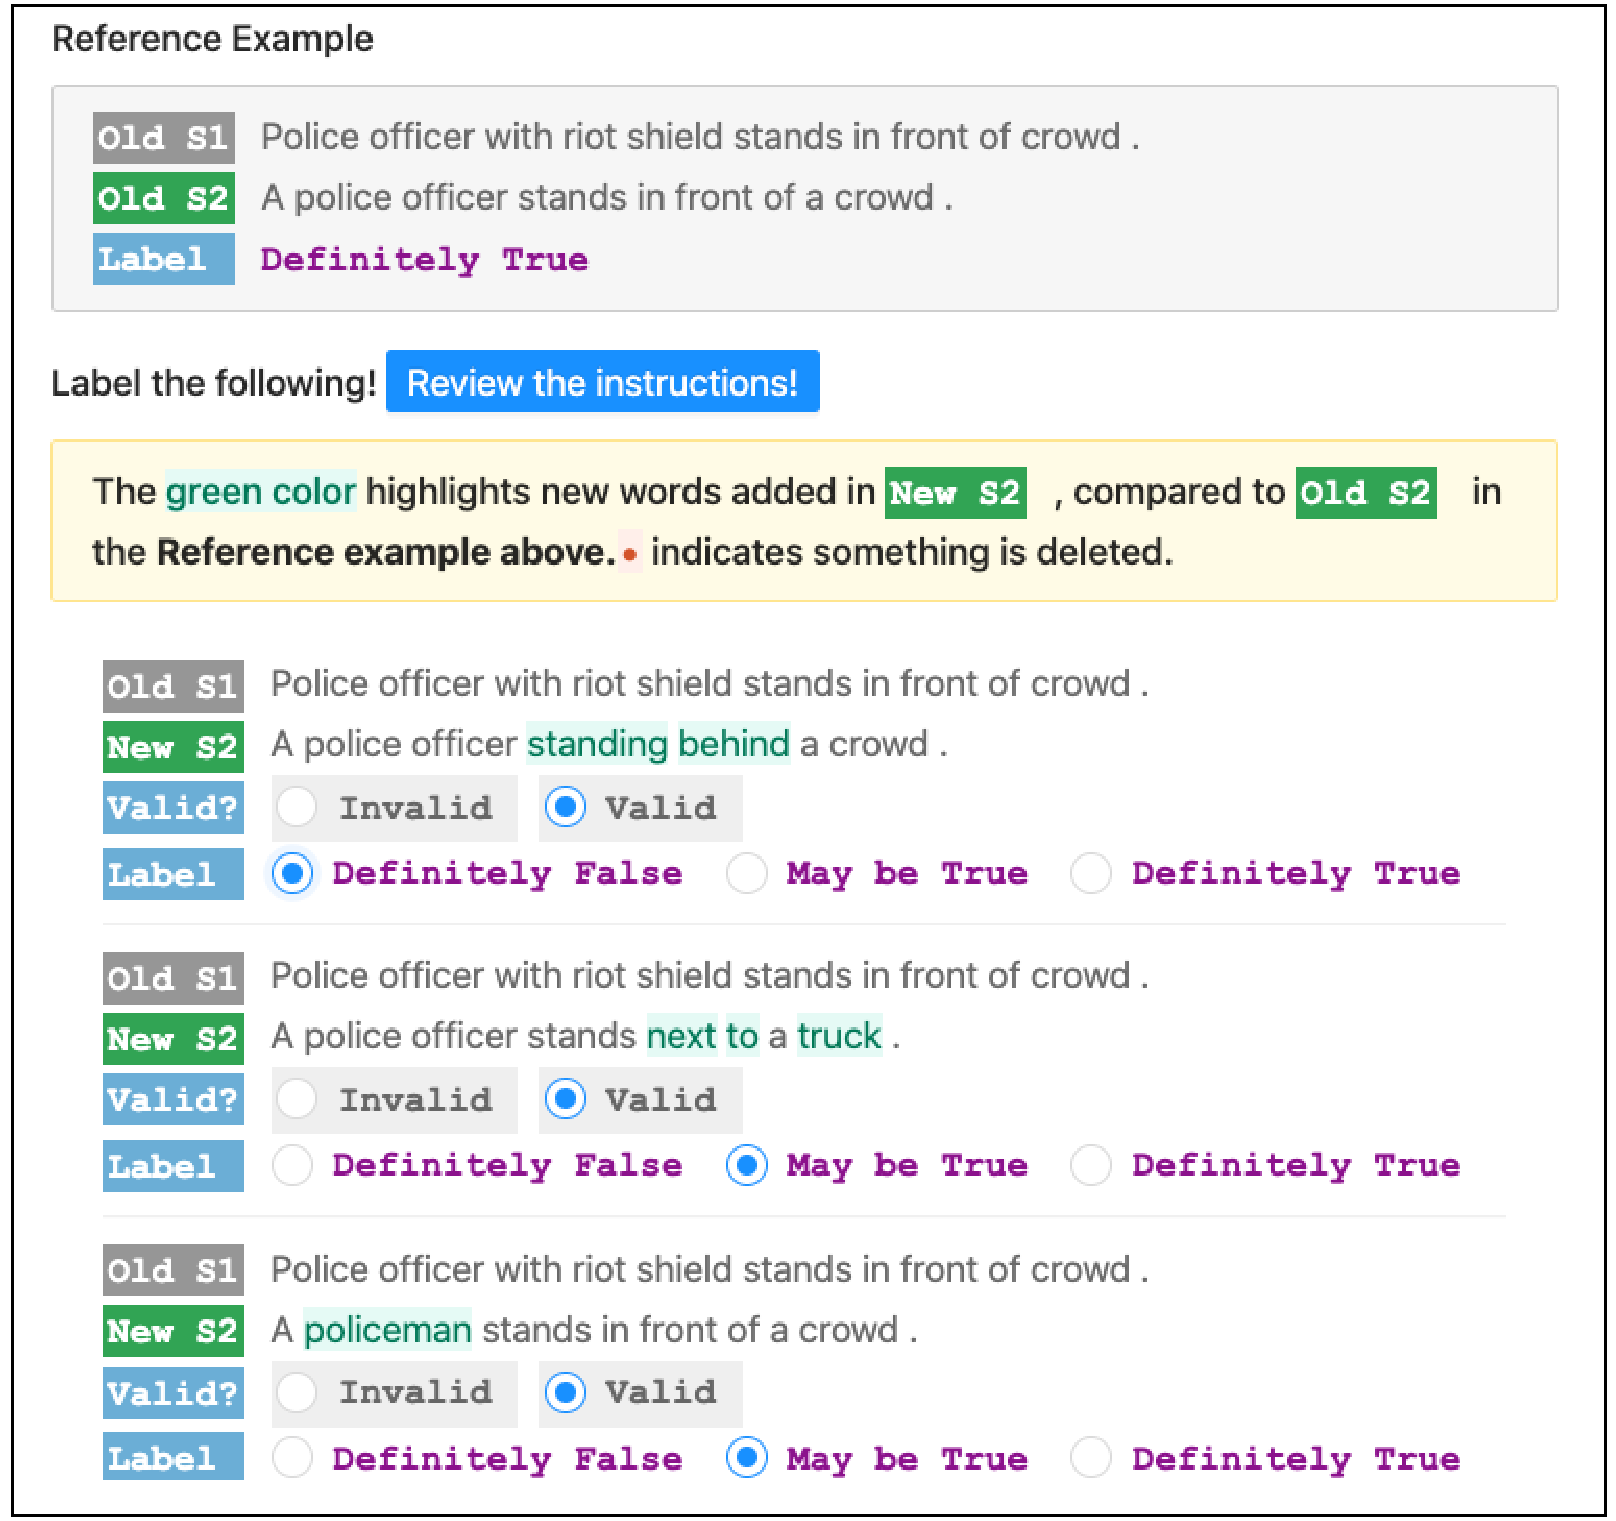
\includegraphics[width=1\columnwidth]{figures/mturk_label}
\vspace{-15pt}
\caption{A sample labeling task: The crowdworkers annotate three perturbations based on their validity and class label, with respect to the original instance. \wts{This is placeholder screenshot. Change width/height ratio, choose a better example}}
\vspace{-10pt}
\label{fig:mturk_instruction}
\end{figure}

\subsection{Contrast Set Evaluation}
\label{subsec:contrast_set}
For each task, we crowd labeled 1,500 perturbations on 500 original examples.
For \qqp and \nli, we only perturbed \emph{duplicate} and \emph{entailment} examples, as it usually take significant changes to flip other labels.
After validity and majority vote filtering, we kept around 400 perturbations on 270 original examples (357 $\xp$ on 252 $x$ for \sst, 423 $\xp$ on 278 $x$ for \nli, 450 $\xp$ on 286 $x$ for \qqp).
Following the contrast set definition, we filter the labeled $\xp$-s to only keep $\xp$-s whose groundtruth label is different from $x$'s, resulting in 100-200 perturbed instances: 106 $\xp$ on 88 $x$ for \sst, 276 $\xp$ on 202 $x$ for \nli, 243 $\xp$ on 185 $x$ for \qqp.
\nli was the easiest to change labels, with a flip rate of $60\%$, and \sst was the hardest (only flipping 36.9\%).

We tested opensourced models on HuggingFace~\cite{Wolf2019HuggingFacesTS}:
DistilBERT fintuned on SST-2 for \sst\footnote{\url{https://huggingface.co/distilbert-base-uncased-finetuned-sst-2-english}},
RoBERTa fintuned on MNLI for \nli\footnote{\url{https://huggingface.co/roberta-large-mnli}},
and BERT fintuned on QQP for \qqp\footnote{\url{https://huggingface.co/textattack/bert-base-uncased-QQP}},
We report model accuracies on the full test set, the original examples set for collecting perturbations, and the perturbed, contrast set.
We also report consistency, \ie the percentage of the perturbation groups for which a model's predictions are correct for all examples (including the original $x$)~\cite{li2020linguistically}.
Table~\ref{table:contrast_set_result} shows that all the models perform worse on the contrast set.

\begin{table}
\small
\centering
\setlength{\tabcolsep}{4pt}
\begin{tabular}{c c c c c}
\toprule
\textbf{Task} & \textbf{Dev.} & \textbf{Orig.} & \textbf{Con.} & \textbf{Consist.} \\ 
\midrule
\sst & 91.1 & 93.2 & 84.0 (-9.2) & 75.0 \\
\qqp & 90.9 & 88.1 & 75.7 (-12.4) & 60.5 \\
\nli & 86.5 & 91.6 & 72.3 (-19.3) & 56.4 \\
\midrule
% the baseline
% \nli & 86.5 & 80.6 & 78.6 (-19.3) & 30.4 \\
% using a imdb model
% imdb_contrast_test 96.7 / 89.1 / 86.1
% imdb_iclr_test 96.7 / 91.0 / 87.9
% using a sst-2 model
% imdb_iclr_test 91.3 / 89.5 / 81.4
% imdb_iclr_test 89.5 / 87.3 / 77.3
\bottomrule
\end{tabular}
\caption{Perturbations as contrasts sets, with accuries on the original development set, the examples used for perturbations (\emph{Orig.}), the perturbed-to contrast sets (\emph{Con.}), and the consistency between \emph{Orig.} and \emph{Con.} \wts{Add baseline -- How do the model perform on existing contrast sets? }}
\label{table:contrast_set_result}
\end{table}
%\end{comment}


%%%%%%%%%%%%%%%%%%%%%
\TableAugSST
\TableAugNLI
%%%%%%%%%%%%%%%%%%%%%

\subsection{Counterfactual Data Augmentation}
\label{subsec:augmentation}
\paragraph{Filtering.}
Because invariant perturbations can also potentially improve model stability, we keep all the valid perturbations for one $x$, as long as at least one of them flips the groundtruth label.

\paragraph{Baselines.}
For each augmented model (\maug) in this section, we include $m$ perturbations, as well as $n$ examples sampled from the original dataset (the base examples of the perturbations will always be included).
As a baseline, we also train compensation models (\mcomp).
These models have the same $n$ original examples as their corresponding augmented models; However, the $m$ perturbations are replaced by another $m$ original samples.
Comparing with these models help highlight the effectiveness of perturbations with respect to adding the same amount of original data. 

\paragraph{Model.}
We finetune \texttt{roberta-base} models~\cite{liu2019roberta} provided by HuggingFace Transformers~\cite{Wolf2019HuggingFacesTS}.
For each data sample, we train the models with four random seeds, and report the averaged metrics. 
For each run, we heuristically picked initial learning rates 1e-5, 2e-5, 2e-5 for \sst, \nli and \qqp, respectively, trained 20 epochs, and selected the epoch that had the highest accuracy on the corresponding validation set (1/5 of the training data size, with the same ratio of original and perturbation examples.)
\wts{Double check the reproducibility requirement to see if there's anything missing. And should I move the whole section to appendix?}
For each given $(m,n)$, we create three different samples of training data, and report the average and the variance of the samples. 
\wts{Fix the naming later: should I say perturbations, counterfactuals, or something else?}



%\textbf{Results.}
\subsubsection{Augmentation Results}
\wts{This can also be at the end.}
As detailed below, we observe that, compared to adding the same amount of original data: 
(1) The perturbation augmentation helps improve models' generalization accuracies on out-of-domain datasets, challenge sets and contrast sets, as well as CheckList testing results~\cite{checklist:acl20}.
Critically, the improvement maintains even when the augmentation size is small (\eg when $m/n<10\%$).
\wts{change number.}
(2) Meanwhile, it can maintain the in-domain accuracy.
(3) However, random samples of augmentation may be insufficient. Rather, the data should be selected based on particular data slices that needs improvements. 
Active learning might be a promising future direction.
\wts{Maybe active learning should be in future work.}
(4) The ratio of the original data and the new data is also important. Flipping out too much original data may hurt the model performance.
\wts{See from the results if we want this takeaway.}




\begin{figure}[t]
\centering
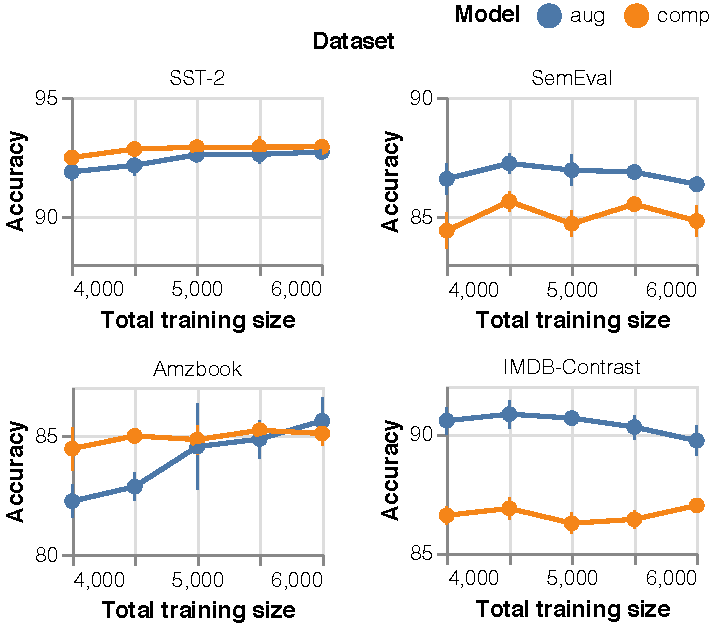
\includegraphics[width=1\columnwidth]{figures/sst_trend}
\vspace{-15pt}
\caption{The accuracy trend on four representative datasets, as the total training datasize ($m+n$) changes. The orange line shows an augmentation of $m=2k$ perturbations, and the blue one represents the corresponding \mcomp.
Therefore, when $m+n=4k$, we have $m=n=2k$ on the orange line; whereas when $m+n$ increases to $6k$, we have $n=2m=4k$.
Though the perturbation remains useful on SemEval across all $m+n$, it appears too many perturbations may be harmful (from SST-2 and Amzbook), yet too few may be ineffective (from IMDB-Contrast.)
}
\vspace{-10pt}
\label{fig:sst_trend}
\end{figure}

\wts{Is it better to organize this part as in the general exam, i.e. just by the observations?}
\paragraph{\sst.}
 Similar to \citet{kaushik2019learning}, we evaluate \sst model's generalization accuracy on out of domain datasets, including review datasets (IMDb movie review~\cite{maas2011learning}, Yelp~\cite{asghar2016yelp} and Amazon~\cite{ni2019justifying}), Twitter dataset (Senti140~\cite{go2009twitter} and SemEval 2017~\cite{rosenthal2017semeval}), and contrast sets on IMDB movie review (IMDB Contrast~\cite{kaushik2019learning} and IMDb Contrast-CAD~\cite{gardner2020contrast}).
For each dataset, we randomly selected up to 2,000 examples.
\wts{check number.}
As shown in Table~\ref{table:aug_sst}, compared to the same amount of original data, by adding $m=2k$ perturbations to $n=4k$ originals, we were able to maintain the  in-domain accuracy on SST-2, as well as the out-of-domain accuracies on reviews (Amzbook, Yelp, IMDB.)
Meanwhile, \maug improves on the out-of-domain Twitter data (Senti140, SemEval), likely because their distribution are less similar to SST-2 than the reviews.
The model also improves on the the contrast set and the CDA data.

%, when we train models with different number of original data $n$
\wts{Am I reading too much into these results? We can also cut the figure/paragraph...}
Interestingly, different datasets react differently to the $m/n$ ratio.
As shown in Figure~\ref{fig:sst_trend}, when adding the same $m=2k$ perturbations to $n=2k$ to $4k$ original instances, we observe three major trends:
(1) The perturbation remains effective on some datasets (SemEval and Senti140), 
(2) the effectiveness of the perturbation can decrease on some datasets as the perturbation takes less ratio, as the marginal positive (negative) slopes of \mcomp (\maug) in IMDB-Contrast indicates,
(3) When the proportion of perturbations is large, it may hurt model performance on some datasets (Amzbook; SST-2 and Yelp also follow the trend, though much less observable).
We suspect that flipping out too much original data may decrease the diversity of vocabulary and syntactic structures, which results in the decreased model performance.




\paragraph{\nli.}
% m=20k, n=1574
Unlike the gain in \sst, when we added random perturbations, we did not observe any improvement on any datasets (denoted as \texttt{aug-r} in Table~\ref{table:aug_nli}).
We suspect a large number of perturbations are teaching the model patterns that it has already learned (\eg perturbations contrasting subjects ``man'' and ``woman'' may be unnecessary.) 
%For example, While flipping the from ``man'' to ``woman'' is a perfectly valid lexical change, the existing \dnli dataset already cover data points contrasting the subject of two sentences.
Instead, we prioritize perturbations that can improve error cases identified by \citet{kim2019probing} (we refer to the dataset as DNC).
\wts{Instances that are different from both the existing data and the already labeled perturbation will be more likely to contain patterns that are rarely seen by the model. 
In other words, these instances should better compensate the training space or the testing space.}
We follow \citet{chen2019slice}'s data slicing strategies, and gathered data points with prepositions, comparative adjectives, negations, quantifiers, and antonyms\footnote{We extended their Appendix A.1 to include more cases of \eg comparative adjectives or negations using POS tags and parsing structures.}.
We further enforce changes on the corresponding patterns by blanking out the identified patterns, so to enforce changes on the corresponding patterns.
For example, to hopefully get an augmentation focused on prepositions like \exinline{His surfboard isB \swap{beneath}{lying on} him}, we first filter examples with prepositions like ``beneath'', and generate blanked sentences like \exinline{\ctrltag{[resemantic/lexical]} His surfboard is \BLANK him.}
\footnote{All examples shown are actual generations of the model. \wts{Move this footnote to where it first occurs.}}

As a result, \maug was able to perform better on DNC (Table~\ref{table:aug_nli}), while maintaining in-domain (on SNLI test set) and out-of-domain accuracies (on MNLI matched and mismatched~\cite{williams-etal-2018-broad}).
%As shown in Figure~\ref{}, higher ratios of augmentation data is more useful. 
%That said, 
Just adding $N\%$ data is sufficient to boost the performance.% to some extent.
Because DNC includes pairs of probing examples (one from the original MNLI and one manually probed for a given linguistic pattern), we can safely conclude that the model did not overfit to a new pattern (i.e., it does not improve on \exinline{lying on} by sacrificing performances on \exinline{beneath.})
The model also performs better on some other challenge sets that are not our initial improvement targets~\cite{naik2018stress, glockner-etal-2018-breaking, wang2018glue}.

\TableAugQQP

\paragraph{\qqp.}
We validate the models using tests defined in CheckList.
As a behavioral testing framework, CheckList defines multiple tests, and measures models' linguistic capabilities using the failure rates of each test.
Because failure rates are more sensitive than accuracy, we say a model capability is affected, if the failure rate of a test changes (increases or decreases) more then 5\% (\eg failure rates going from 20\% to 21\% is insignificant), and the delta accounts for 10\% (\eg failure rates decreasing 8\% from 100\% to 92\% does not count.)

Similar to \nli, we focus on data slices whose perturbations may be more helpful on failed tests identified in CheckList, \eg the entity orders (slicing on examples with multiple entities, and \ctrltag{shuffle} them).
%, temporal information (\eg find examples with \exinline{before} and \BLANK it to hopefully get \exinline{after}

Augmenting $n=20,000$ original examples with $m=1,911$ perturbations, we reduced model failure rates on 11 tests (out of the 28 failed ones, with the failure rate of \mcomp $>20\%$), and increased that for 2 tests.
Meanwhile, the models have similar accuracies on the test set ($84.5 \pm 0.6$ for \maug, and $84.7 \pm 1.0$ for \mcomp).
Some sample tests are in Table~\ref{table:aug_qqp}.
In most cases, the gain on one test does not hurt its counterparts (\eg we get gains on all tests related to entity ordering.)
However, we did see one potential overfitting: While the model gets significantly better on  \texttt{more X $\not\eq$ less X}, it sacrifices the performance on \texttt{more X $=$ less antonym(X)}.
Future work should further strategize the sampling, such that the augmentation distributes more equally across various related or contrasting sub-cases. 



\begin{comment}
For testing on other datasets, we use a random subset (2000 examples) of the test sets of Amazon Reviews [45], Semeval 2017 (Twitter data) [55], and Yelp reviews [77] similarly to [34].
from Learning What Makes a Difference from Counterfactual Examples and Gradient Supervision
	
\end{comment}
